\chapter{Evaluación y pruebas}\label{evaluacion}

En este capítulo se realizarán las pruebas al sistema. Para ello, a partir de un archivo que contenga una traza de tráfico, se 
analizará con el módulo creado, de forma que se compruebe que se crea el registro correspondiente y que este contiene los flujos 
emparejados.

\intro Se añadirán capturas de pantalla en las que se vea claramente que todo funciona como debería, así mismo, se podrán comprobar 
los registros que se creen en el repositorio de GitHub \citep{repo}.

\section{Establecer las variables}

Lo primero que se hará, será establecer las variables \textit{k1} y \textit{k2}. Estas se definen de forma global al principio 
del módulo. Cómo ya se vio anteriormente, en la explicación de la ecuación \ref{ecug}, sus valores estarán comprendidos entre 0,1 y 
10000. Como se puede ver, en la Figura \ref{fig.variables}, para las pruebas se han establecido los valores en 1 y 100.

\begin{figure}[H]
  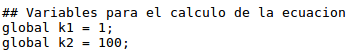
\includegraphics[width=0.6\textwidth]{imagenes/variables.png}
  \centering
  \caption{Valores de las variables \textit{k1 y k2}.}\label{fig.variables}
\end{figure}

\intro A su vez, también será necesario definir el umbral que servirá para descartar o aceptar emparejamientos. Como se puede ver en 
la Figura \ref{fig.definirumbral}, en el caso de estas pruebas el valor será de 1.

\begin{figure}[H]
  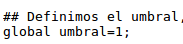
\includegraphics[width=0.3\textwidth]{imagenes/definirumbral.png}
  \centering
  \caption{Valor de la variable \textit{umbral}.}\label{fig.definirumbral}
\end{figure}


\section{Prueba del módulo}

A continuación, se realizará una prueba del módulo, con las variables anteriormente descritas, para comprobar que todo funciona 
correctamente.

\intro Como se puede ver en la Figura \ref{fig.terminal}, para lanzar el módulo, será necesario indicar el archivo que se va a 
analizar.

\begin{figure}[H]
  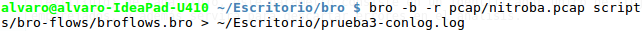
\includegraphics[width=1\textwidth]{imagenes/terminal.png}
  \centering
  \caption{Lanzamiento del módulo para realizar el análisis.}\label{fig.terminal}
\end{figure}

\intro Cabe destacar, que para la depuración se muestran mensajes por terminal. Estos son escritos en un archivo mediante el carácter \textit{mayor que}, de forma que se pueda realizar búsquedas sobre ellos. En la Figura \ref{fig.salida} se puede ver una muestra de estos mensajes,en los cuales se muestra el \textit{uid} de los dos flujos, el número de IP's coincidentes y los puertos de ambos flujos.

\begin{figure}[H]
  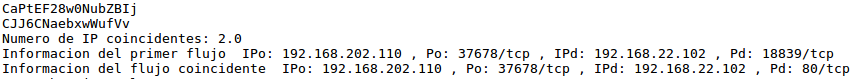
\includegraphics[width=1\textwidth]{imagenes/salida.png}
  \centering
  \caption{Muestra de los mensajes de depuración.}\label{fig.salida}
\end{figure}

\intro En el registro que se crea cada vez que se ejecuta el análisis, además de las IP's y los puertos, también se muestran los 
\textit{uid} de cada flujo, este parámetro consiste en un identificador único de flujo. Esto ayudará a identificar los flujos que son 
emparejados y además, servirá para descartar errores en el análisis.

\intro En la Figura \ref{fig.lognitroba}, se puede comprobar el registro que se genera al analizar un archivo. En este caso, el 
archivo analizado ha sido \textit{nitroba.pcap}, cuyo peso es de 56,2 MB, el cual se encuentra accesible desde la web de Bro. Esta 
traza se corresponde con un escenario de prueba realizado por una universidad sudafricana. 

\begin{figure}[H]
  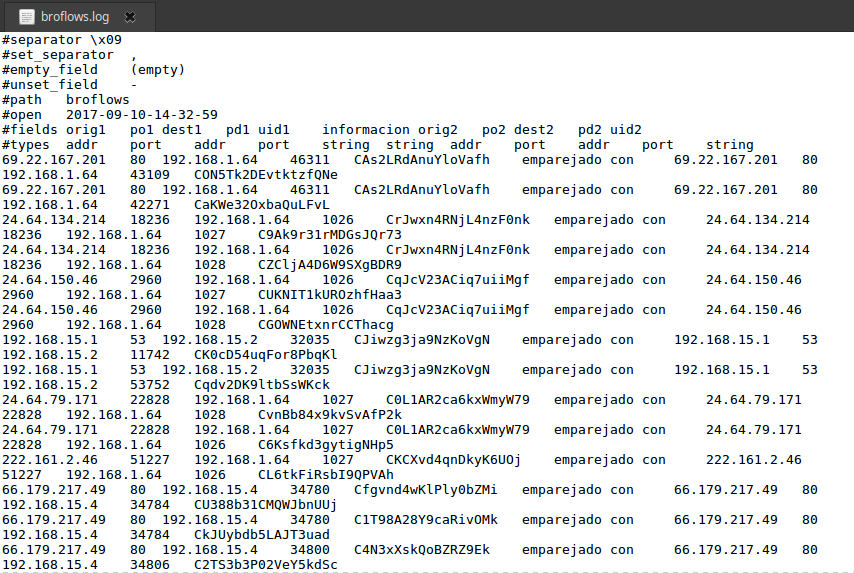
\includegraphics[width=0.9\textwidth]{imagenes/lognitroba.png}
  \centering
  \caption{Log del archivo \textit{nitroba.pcap}.}\label{fig.lognitroba}
\end{figure}

\intro En el registro se pueden ver los flujos emparejados. Al trabajar con una traza pequeña, cabe esperar que sean pocos los 
resultados, en cuanto a número de flujos emparejados. Este tipo de archivos son ideales para realizar las pruebas, pues tarda muy poco 
el sistema en analizarlos, siendo en este caso 1 segundo el tiempo utilizado.

\intro En la Figura \ref{fig.dosflujosemparejados}, se encuentran dos emparejamientos que pertenecen a la misma clase. Esto se puede 
comprobar, ya que el primer flujo tiene el mismo \textit{uid} y los flujos con los que se empareja no.

\begin{figure}[H]
  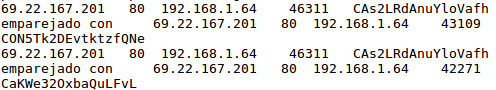
\includegraphics[width=1\textwidth]{imagenes/dosflujosemparejados.png}
  \centering
  \caption{Dos flujos emparejados.}\label{fig.dosflujosemparejados}
\end{figure}

\intro Por lo tanto, con esto se puede afirmar que el módulo empareja de forma adecuada los flujos.

\intro En cuanto al borrado de flujos, en la Figura \ref{fig.borrado}, se puede ver que el \textit{uid} de un flujo activo solo existe 
dos veces, siendo borrado de memoria después de esas comparaciones. Por lo tanto, se puede afirmar que el módulo borra de forma 
adecuada los flujos cuando ya no los necesita.

\begin{figure}[H]
  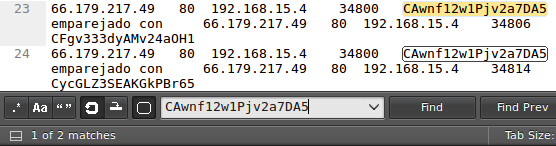
\includegraphics[width=1\textwidth]{imagenes/borrado.png}
  \centering
  \caption{Borrado de flujos.}\label{fig.borrado}
\end{figure}

\intro Además, la única información accesible es la que está en el registro, por lo que no se entra dentro de los paquetes y se 
garantiza la privacidad.

\section{Escenarios reales}

Una vez que se ha comprobado que todo funciona de forma correcta con un archivo pequeño, se pasará a analizar un archivo más grande, 
correspondiente a un escenario real. En este caso se trata de \textit{maccdc2012\_00004.pcap}, correspondiente al \textit{National 
CyberWatch Mid-Atlantic Collegiate Cyber Defense Competition} o \textit{MACCDC} \cite{maccdc}. En este archivo se encuentra el tráfico 
de un día y ocupa cerca de 1.1 GB.

\intro En la Figura \ref{fig.logmaccdc}, se puede ver que al realizar el análisis con el módulo, se obtiene un registro mucho más 
extenso. De hecho, tarda cerca de 50 minutos en realizarlo, frente al segundo que tardaba el análisis del archivo anterior.

\begin{figure}[H]
  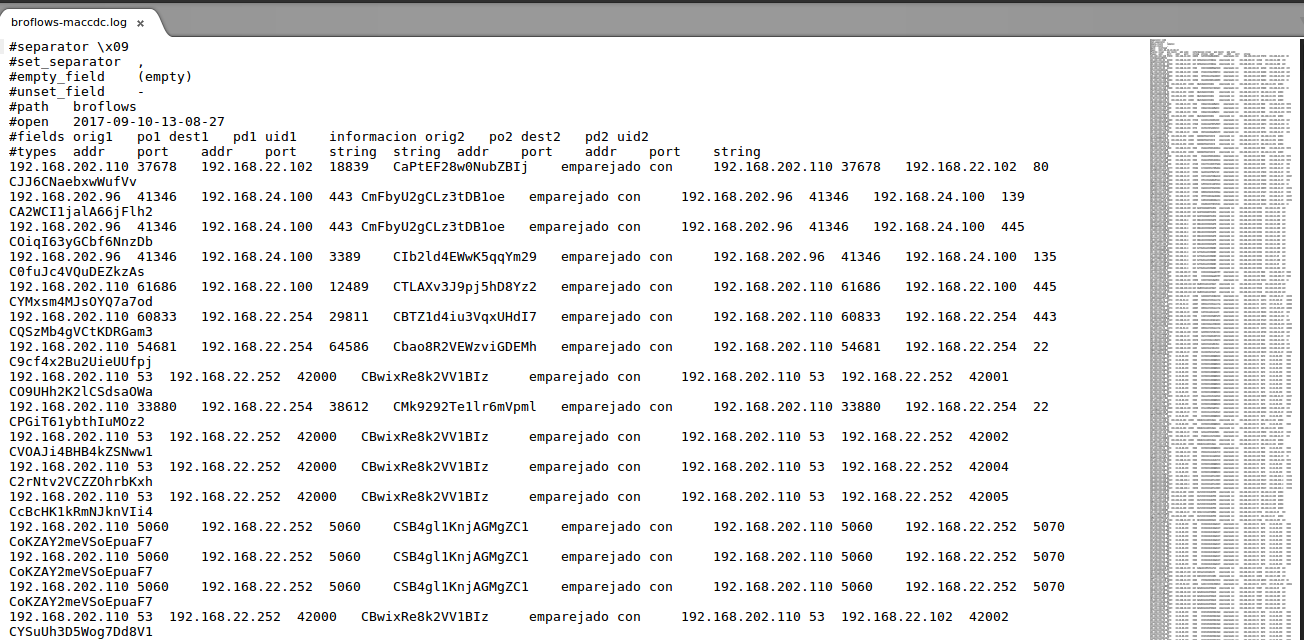
\includegraphics[width=1\textwidth]{imagenes/logmaccdc.png}
  \centering
  \caption{Log del archivo \textit{maccdc2012\_00004.pcap}.}\label{fig.logmaccdc}
\end{figure}

\intro Mientras que en el análisis anterior se llegaba como mucho a emparejar tres flujos, en este se pueden llegar a obtener unos 8 
flujos emparejados, como se ve en la Figura \ref{fig.flujosemparejados}. Cabe destacar, que estos resultados variarán en función de los valores que se le asignen a los parámetros y al umbral.

\begin{figure}[H]
  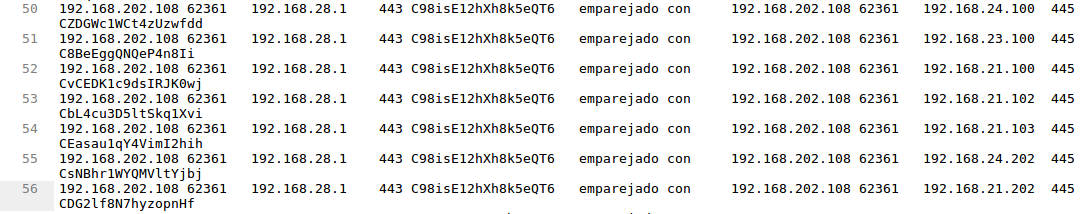
\includegraphics[width=1\textwidth]{imagenes/flujosemparejados.png}
  \centering
  \caption{Flujos emparejados.}\label{fig.flujosemparejados}
\end{figure}

\intro Y de nuevo, si se realiza una búsqueda usando el \textit{uid} del primer flujo, se verá que no se muestra más veces, por lo que 
se realiza el borrado de la tabla de activos correctamente.

\intro Por lo tanto, vemos que también es escalable siendo analizado en este apartado un archivo de 1.1 GB, y en el anterior un 
archivo de 0.05 GB. Obviamente, el tiempo no se mantiene estable, pues es imposible analizar tanta información en un segundo. Pero, este archivo contiene el tráfico de todo un día, por lo que un análisis de esa cantidad de tráfico en menos de 50 minutos, es algo 
aceptable.
